% !TeX spellcheck = en_US	

\documentclass[10pt,journal,compsoc]{IEEEtran}
\usepackage{graphicx}
\usepackage[ruled, linesnumbered]{algorithm2e}
\usepackage{url}
\usepackage{epstopdf}
\usepackage{indentfirst}
\usepackage[tight,footnotesize]{subfigure}
\usepackage{amsmath}
\usepackage{amssymb}
\usepackage{multirow}
\usepackage{color}
\usepackage{enumerate}

\newtheorem{theorem}{Theorem}[section]
\newtheorem{lemma}[theorem]{Lemma}
\newtheorem{observation}[theorem]{Observation}
\newtheorem{corollary}[theorem]{Corollary}
\newtheorem{formula}[theorem]{Formula}

% *** CITATION PACKAGES ***
\ifCLASSOPTIONcompsoc
\usepackage[nocompress]{cite}
\else
\usepackage{cite}
\fi

\begin{document}

\title{Building and Checking Suffix Array Using Induced Sorting Method}

\author{Yi~Wu,
	Ge~Nong,
	Wai~Hong~Chan,
	and~Bin~Lao
	\IEEEcompsocitemizethanks{
		\IEEEcompsocthanksitem Y. Wu, G. Nong (corresponding author) and B. Lao are with the Department of Computer Science, Sun Yat-sen University, Guangzhou 510275, China. E-mails: wu.yi.christian@gmail.com, issng@mail.sysu.edu.cn, Laobin@mail3.sysu.edu.cn.
		
		\IEEEcompsocthanksitem Wai Hong Chan (corresponding author) is with the Department of Mathematics and Information Technology, The Education University of Hong Kong, Hong Kong. E-mail: waihchan@ied.edu.hk.
}}% <-this % stops a space


\IEEEtitleabstractindextext{% 
\begin{abstract}

Suffix array~(SA) can be built by the induced sorting~(IS) method on both internal and external memory models. We propose two methods that enable any IS suffix sorter to build and check an SA simultaneously. The first method can check both suffix and longest common prefix~(LCP) arrays for strings drawn from constant alphabets, while the second method is applicable to checking SA for strings of any alphabets. By combining our methods with the Karp-Rabin fingerprinting function, we design two probablistic algorithms that perform verification with a neligible error probability. These algorithms are rather lightweight in terms of time and space. Particularly, the algorithm designed by the second method only takes linear time and constant space when running in external memory. For a further study, we integrate the checking algorithm designed by the second method into the existing suffix sorter DSA-IS to evaluate the checking overhead, where the time, space and I/O consumptions for verification are considerably smaller than that for construction in the experiments. This convinces us that the proposed checking methods, together with the state-of-the-art IS suffix sorters, could constitute efficient solutions for both construction and verification. 

\end{abstract}

% Note that keywords are not normally used for peerreview papers.
\begin{IEEEkeywords}
Suffix and LCP arrays, construction and verification, external memory.
\end{IEEEkeywords}}


% make the title area
\maketitle

\IEEEdisplaynontitleabstractindextext

\IEEEpeerreviewmaketitle

\section{Introduction}\label{sec:introduction}

A suffix array can be built in linear time and space by the internal-memory algorithm SA-IS~\cite{Nong11}. According to the IS principle, the relative order of two unsorted suffixes is determined by sequentially comparing the heading characters and the sorted succeeding suffixes starting with their second characters. Recently, the IS method has been applied to designing three disk-based suffix sorting algorithms eSAIS~\cite{Bingmann12}, DSA-IS~\cite{Nong15} and SAIS-PQ~\cite{Liu15}, which have a better time complexity than the other alternatives~(e.g., DC3~\cite{Dementiev2008a}, bwt-disk~\cite{Ferragina2012}, SAscan~\cite{Karkkainen2014} and pSAscan~\cite{Karkkainen2015}) but suffer from a bottleneck due to the large disk space for obtaining the heading characters of unsorted suffixes and the ranks of their successors in a disk-friendly way. More specifically, the average peak disk use to construct an SA encoded by 40-bit integers for pSAscan is $7.5n$, while that for eSAIS, DSA-IS and SAIS-PQ are $24n$, $20n$ and $15n$, respectively. The poor space performance is mainly because that the current programs for these algorithms fail to free the disk space for temporary data even when the data is no longer to use. A dramatic improvement can be achieved by splitting a file into multiple pieces and deleting each piece immediately when the temporary data in it is not needed any more. This technique has been used to implement a new IS suffix sorting algorithm fSAIS~\cite{Karkkainen2017}. As reported, the engineering of fSAIS consumes no more than $8n$ disk space for constructing an SA encoded by 40-bit integers, indicating a great potential for optimizing our programs for DSA-IS and SAIS-PQ. 

A constructed SA should be checked to avoid computation errors caused by implementation bugs and/or hardware malfunctions. Currently, the software packages for DC3 and eSAIS provide users a checker designed by the method proposed in~\cite{Dementiev2008a}. The overhead for this checker is rather high because it takes two external-memory sorts for arranging $\mathcal{O}(n)$ fixed-size tuples according to their integer keys. Against the background, we propose in this paper two methods that enable any IS suffix sorter to check an SA when it is being built. The first method can check both suffix and LCP arrays for strings drawn from constant alphabets, while the second method can check SA for strings drawn from any alphabets. We augment these methods with the Karp-Rabin fingerprinting function~\cite{Karp1987} to design two probabilistic algorithms, in terms of that their checking results are wrong with a negligible probability. These algorithms are rather lightweight in terms of time and space. Particularly, the algorithm designed by the second method only takes linear time and constant space to run using external memory. For a further study, we integrate this algorithm into DSA-IS to evaluate its checking overhead, where the design of DSA-IS has been adapted by new substring sorting and naming methods for a better performance. As demonstrated in our experiments, the time, space and I/O consumptions for verification by this algorithm are negligible to that for construction by the adapted DSA-IS. We are convinced that the proposed SA checkers, together with the state-of-the-art IS suffix sorters, could constitute efficient solutions for both construction and verification.

The rest of this paper is organized as follows. Section~\ref{sec:preliminaries} introduces some basic notations and symbols. Section~\ref{sec:builder} gives an overview of IS suffix sorting algorithms and the details of new substring sorting and naming methods. Section~\ref{sec:checkers} describes the ideas of checking methods and algorithms. Sections~\ref{sec:experiments} and~\ref{sec:conclusion} show the experimental results and the concluding remarks, respectively.

\section{Preliminaries}~\label{sec:preliminaries}

Given a string $x[0,n)$ drawn from a full-ordered alphabet $\Sigma$, we assume the ending character $x[n - 1]$ to be unique and lexicographically smaller than any other characters in $x$. For convenience, we denote by ${\sf suf}(i)$ and ${\sf sub}(i, j)$ the suffix running from $x[i]$ to $x[n-  1]$ and the substring running from $x[i]$ to $x[j]$, respectively. The following notations are also used in our presentation.

Characters in $x$ are classified into two categories: L-type and S-type. We say $x[i]$ is S-type if (1) $i = n - 1$ or (2) $x[i] = x[i + 1]$ and $x[i + 1]$ is S-type; otherwise $x[i]$ is L-type. Further, if $x[i]$ and $x[i - 1]$ are respectively S-type/L-type and L-type/S-type, then $x[i]$ is also called S*-type/L*-type. We use an array $t$ to record the type of all the characters in $x$, where $t[i] = 1$ or $0$ if $x[i]$ is S-type or L-type, respectively. A substring or suffix is of the same type as its heading character. In this paper, we only consider substrings ending with an S*-type character.

Given two characters $x[i]$ and $x[i + 1]$, we say $x[i]$ is the predecessor of $x[i + 1]$ and $x[i + 1]$ is the successor of $x[i]$. Accordingly, we define the predecessor-successor relationship between ${\sf suf}(i)/{\sf sub}(i, j)$ and ${\sf suf}(i + 1)/{\sf sub}(i + 1, j)$.

We partition $x$ into S*-type substrings and replace each substring with its name to produce the reduced string $x_1$, where the name indicates the rank of the corresponding S*-type substring among all. 

The suffix array $sa$ indicates the lexical order of all the suffixes in $x$, where $sa[i]$ records the starting position of the $(i + 1)$-th smallest suffix. We also define the suffix array $sa_1$ for $x_1$ following the same way. 

The LCP array $lcp$ indicates the LCP-values of all the neighboring suffixes in $sa$, where $lcp[0] = 0$ and $lcp[i] = \ell$ for $i \in [1, n)$, where $\ell$ is the length of longest common prefix of ${\sf suf}(sa[i])$ and ${\sf suf}(sa[i - 1])$.

All the suffixes in $sa$ are naturally partitioned into multiple buckets. Each bucket occupies a contiguous interval in $sa$ and contains all the suffixes starting with a certain character. Without loss of generality, we denote by ${\sf sa\_bkt}(c_0)$ the bucket for suffixes starting with $c_0$. Notice that ${\sf sa\_bkt}(c_0)$ can be further divided into two parts, where the left part ${\sf sa\_bkt_L}(c_0)$ and the right part ${\sf sa\_bkt_S}(c_0)$ contain the L-type and S-type suffixes, respectively. We also partition $lcp$ into buckets such that ${\sf lcp\_bkt}(c_0)$, ${\sf lcp\_bkt_L}(c_0)$ and ${\sf lcp\_bkt_S}(c_0)$ record the LCP-values of suffixes in ${\sf sa\_bkt}(c_0)$, ${\sf sa\_bkt_L}(c_0)$ and ${\sf sa\_bkt_S}(c_0)$, respectively.

Let $n_1 = \|x_1\|$, we use $sa^*[0, n_1)$ and $lcp^*[0, n_1)$ to denote the suffix and LCP arrays for S*-type suffixes in $x$, respectively. Specifically, $sa^*[i]$ records the starting position of the $(i + 1)$-th smallest S*-type substring, while $lcp^*[i]$ records the LCP-value of ${\sf suf}(sa^*[i])$ and ${\sf suf}(sa^*[i - 1])$.


\section{Builder}~\label{sec:builder}

\subsection{Introduction to IS Suffix Sorting Algorithms} \label{subsec:improvement}

% Algorithm
\begin{algorithm}
	\SetAlgoNoLine
	\KwIn{$x$}
	\KwOut{$sa$}
	
	/* Reduction Phase */ \\
	Sort S*-type substrings by the IS method.
	
	Name the sorted S*-type substrings to produce $x_1$.
	
	~\\
	
	/* Check Recursion Condition */ \\	
	\If{exist two equal characters in $x_1$}{
		
		
		Recursively call the reduction phase on $x_1$.
	}
	
	~\\
	
	/* Induction Phase */ \\
	Sort suffixes by the IS method.
	
	
	\caption{The overview of IS suffix sorting algorithms	.}
	
	\label{alg:1}
\end{algorithm}

As shown in Algorithm~\ref{alg:1}, an IS suffix sorting algorithm first performs a reduction phase to produce the reduced string $x_1$. If there exist two equal characters in $x_1$, then it recursively calls the reduction phase with $x_1$ as input; otherwise, all the S*-type suffixes in $x$ are already sorted and it performs an induction phase to produce the final $sa$. During the execution of two phases, the order of substrings/suffixes is determined by comparing the heading characters and the ranks of their successors according to the IS principle. This involves frequent random accesses to $x$ and $sa$ for retrieving the heading characters of unsorted substrings/suffixes and the ranks of their sorted successors. It can be done very quickly if both $x$ and $sa$ are wholly loaded into RAM; otherwise, each disk access takes an individual I/O operation, leading to a severe performance degradation. This problem is solved in DSA-IS by conducting two steps:

\begin{enumerate}[S1]
	\item Split $x$ into blocks and sort substrings/suffixes of each block by calling SA-IS, the heading characters in use are copied to external memory in their access order. \label{dsais_sorting_method:1}
	\item Sort the substrings/suffixes of $x$ by their heading characters and the ranks of their successors. Organize the sorted substrings/suffixes in an external-memory heap and induce their predecessors into the heap according to the IS principle, where the heading characters of the induced substrings/suffixes are retrieved from external memory by sequential I/O operations.\label{dsais_sorting_method:2}
\end{enumerate} 

As shown in Section~\ref{sec:experiments}, our program for DSA-IS requires less disk space than that for eSAIS, but the former runs slower than the latter caused by the large I/O volume for sorting and naming S*-type substrings during the reduction phase. For this, we present new substring sorting and naming methods in the next subsection.

\subsection{Improvements on DSA-IS}

All the S*-type substrings are classified into long and short categories with respect to whether or not containing more than $D$ characters. The new substring sorting method mainly consists of the three steps below:

\begin{enumerate}[S1']
	\item Sort the long of each block by S\ref{dsais_sorting_method:1}. During the process, copy the short to external memory in their sorted order.~\label{dsaism_sorting_method:1}
	
	\item Sort the long of $x$ by S\ref{dsais_sorting_method:2}. During the process, copy the leftmost $D$ characters of the long to external memory in their sorted order.~\label{dsaism_sorting_method:2}
	
	\item Merge the short and long by a multi-way sorter.~\label{dsaism_sorting_method:3}
\end{enumerate}

After the first two steps, the short S*-type substrings of each block and the long S*-type substrings of $x$ are sorted and separately organized as a sequence in external memory. Assume $x$ is split into $k$ blocks, the multi-way sorter in S\ref{dsaism_sorting_method:3}' maintains an internal-memory heap to cache the current smallest of each sequence and continually retrieve the top item from the heap to determine the lexical order of substrings from different sequences. The heap contains at most $k + 1$ substrings at any point of time and it compares any two substrings in $\mathcal{O}(D)$ time by a literal string comparison\footnote{If the leftmost $D$ characters of a long S*-type substring is equal to a short S*-type substring, then the short is lexicographically greater than the long.}. Theoretically, the sorting method has a good performance if the majority of S*-type substrings in $x$ are short with a small $D$. This is commonly satisfied in practice, because the average length of S*-type substrings is typically small in real-world datasets.

In what follows, we describe a method for naming the S*-type substrings during the above sorting process. The key point here is to check equality of two substrings successively popped from the heap in S\ref{dsaism_sorting_method:3}' as fast as possible. If either of the two substrings is short, our solution is to literally compare them in $\mathcal{O}(D)$ time. Otherwise, if both of them are long, then we assign names to all the long S*-type substrings using the technique proposed for SAIS-PQ in S\ref{dsaism_sorting_method:2}' and compare two successively popped long S*-type substrings by their names. This technique is based on the idea that two substrings are of the same name if their heading characters and the names of their successors are both equal\footnote{We refer interested readers to~\cite{Liu15} for more information.}.

The experimental results in Section~\ref{sec:experiments} indicate that, by using the new substring sorting and naming methods, the adapted DSA-IS, called DSA-IS+, only takes half as much disk space as eSAIS. Also, the peak disk use of the program for DSA-IS+ can be further reduced to a level comparable to that of the program for fSAIS.

\section{Checkers}~\label{sec:checkers}

\subsection{Prior Art} \label{sec:checkers:prior_art}

The software packages for DC3 and eSAIS provide users a checker to ensure the correctness of their outputs. The following statements describe the idea behind this checker. 

\begin{lemma} \label{lemma:1}
	For $i, j \in [0, n)$ and $i \ne j$, ${\sf suf}(i) < {\sf suf}(j) \Leftrightarrow (x[i], {\sf suf}(i + 1)) < (x[j], {\sf suf}(j + 1))$.
\end{lemma}

\begin{theorem} \label{theorem:1}
	$sa[0, n)$ is the SA for $x[0, n)$ if and only if the following conditions are satisfied:\\
	(1) $sa$ is a permutation of $[0, n)$. \\	
	(2) ${\sf r_i < r_j} \Leftrightarrow (x[i], r_{i + 1}) < (x[i], r_{j + 1})$ for $ i, j \in [0, n)$ and $i\ne j$, where $r_i$ and $r_j$ represent the ranks of ${\sf suf}(i)$ and ${\sf suf}(j)$ among all the suffixes, respectively. \\
\end{theorem}

\begin{IEEEproof}
	Theorem~\ref{theorem:1} is derived from Lemma~\ref{lemma:1}. The proof is available in~\cite{Dementiev2008a}.
\end{IEEEproof}

This checker performs two passes of integer sorts and each sort involves $n$ fixed-size tuples. When implemented in external memory, it consumes large disk space and I/O volume, resulting in a high checking overhead. For example, we can observe from Section~\ref{sec:experiments} that, the peak disk use and the I/O volume for checking an SA encoded by 40-bit integers are around $26n$ and $53n$, respectively. In this section,  we describe two SA checking methods based on the IS principle, both of them can be seamlessly integrated into any IS suffix sorting algorithm to build and check an SA at the same time.

\subsection{Method A} \label{sec:checkers:method_a}

Given that each S*-type substring is unique in $x$, SA-IS first computes $sa^*$ by sorting the starting positions of all the S*-type suffixes with their ranks indicated by $sa_1$ and then induces $sa$ from $sa^*$ by S\ref{induction_phase:1}''-S\ref{induction_phase:3}'' during the inducting phase.

\begin{enumerate}[S1'']
	
	\item Clear $sa$. Scan $sa^*$ leftward with $i$ decreasing from $n_1 - 1$ to $0$. For each scanned item $sa^*[i]$, insert it into the rightmost empty position of ${\sf sa\_bkt_S}(x[sa^*[i]])$. \label{induction_phase:1}
	
	\item Scan $sa$ rightward with $i$ increasing from $0$ to $n - 1$. For each scanned non-empty item $sa[i]$, insert $sa[i] - 1$ into the leftmost empty position of ${\sf sa\_bkt_L}(x[sa[i] - 1])$ if $t[sa[i] - 1] = 0$.\label{induction_phase:2}
	
	\item Clear ${\sf sa\_bkt_S}(c)$ for $c \in \Sigma$. Scan $sa$ leftward with $i$ decreasing from $n - 1$ to $0$. For each scanned non-empty item $sa[i]$, insert $sa[i] - 1$ into the rightmost empty position of ${\sf sa\_bkt_S}(x[sa[i] - 1])$ if $t[sa[i] - 1] = 1$.\label{induction_phase:3}
	
\end{enumerate}

We illustrate a running example of the above process in Fig.~\ref{fig:example1} and show more details for a better understanding. In line 6, we find the ending position of each bucket and insert the sorted S*-type suffixes into the right part of the corresponding buckets. Afterward, we first find the heading position of each bucket (marked by the symbol $\wedge$) and scan $sa$ rightward for inducing the order of L-type suffixes as following. In lines 8-9, we check $\sf suf(14)$ (marked by the symbol $@$) and find its predecessor ${\sf suf(13)}$ is L-type, thus we put ${\sf suf(13)}$ into the current leftmost empty position in ${\sf sa\_bkt_L}(i)$. To step through $sa$ in this way, we get all the L-type suffixes sorted in line 17. After that, we find the ending position of each bucket and scan $sa$ leftward for inducing the order of S-type suffixes in lines 18-28. When scanning $sa[14]$, we see $x[3]$ is S-type and thus put ${\sf suf(3)}$ into the current rightmost empty position in ${\sf sa\_bkt_S}(i)$. Following the same, we get all the S-type suffixes sorted in line 28.


\begin{figure}[t]
	\centering
	
	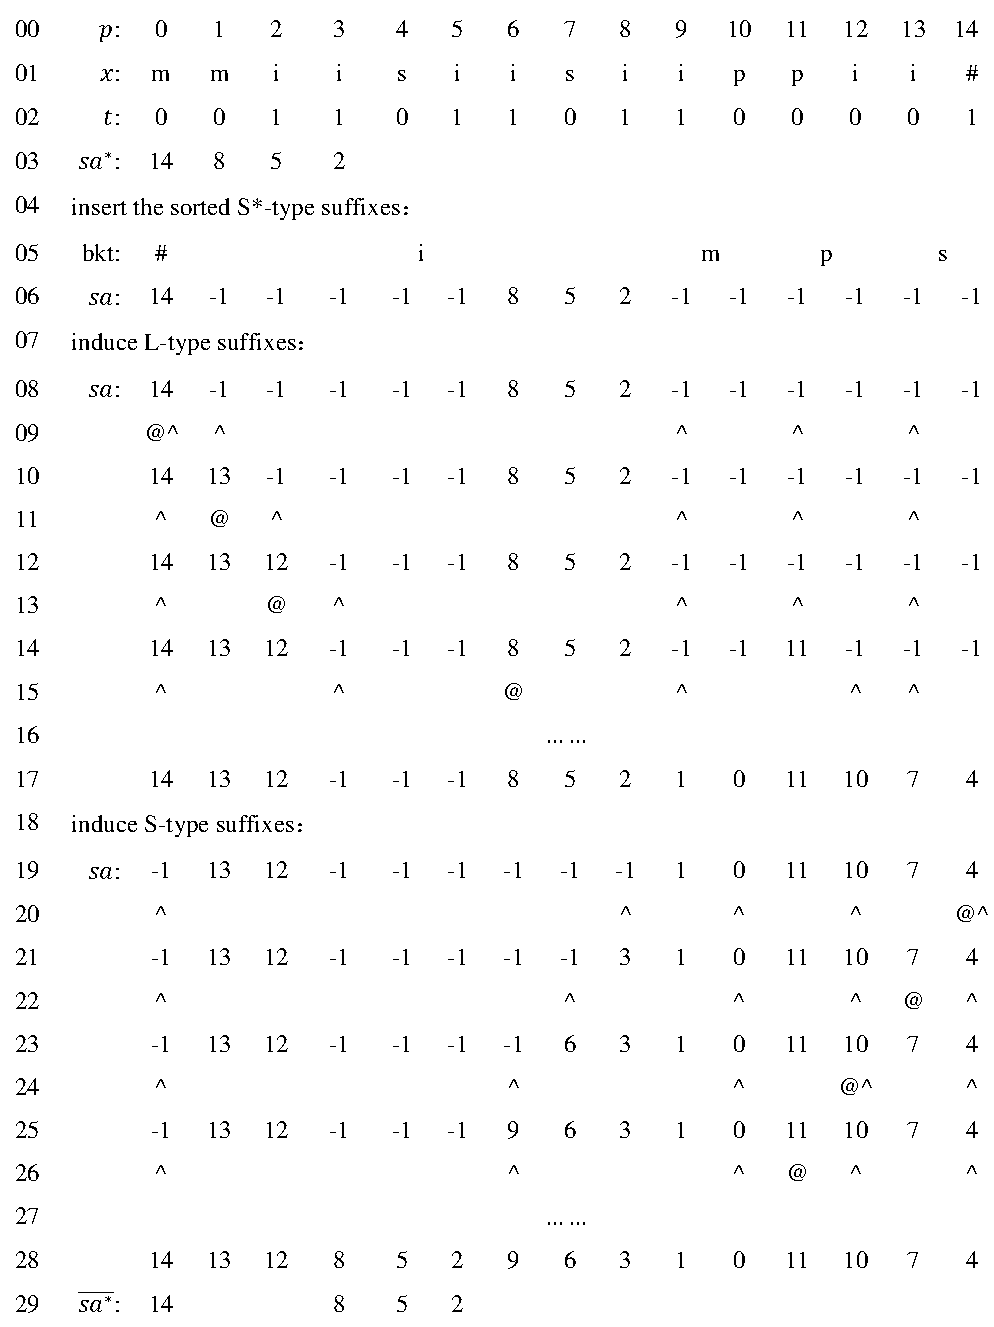
\includegraphics[width = 1\columnwidth]{example.pdf}
	
	\caption{An example for inducing $sa$ from $sa^*$.}
	
	\label{fig:example1}
	
\end{figure}

As stated below, S\ref{induction_phase:1}''-S\ref{induction_phase:3}'' also constitute the sufficient and necessary conditions for a correct $sa$.

\begin{lemma} \label{lemma:3}
	For any IS suffix sorting algorithm, its output $sa[0, n)$ is the SA for the input string $x[0, n)$ if and only if the following conditions are satisfied: \\ 
	(1) $sa^*$ is correct. \\
	(2) $sa[i]$ is equal to the value calculated by S\ref{induction_phase:1}''-S\ref{induction_phase:3}''. \\
	
\end{lemma}

Suppose $sa^*$ is correct\footnote{The correctness of $sa^*$ can be checked by a sparse SA checker, such as~\cite{wu2017}. It should be noticed that the checking processes for $sa^*$ and $sa$ can be executed in parallel.}, this lemma suggests a method to check $sa$ when it is induced from $sa^*$ during the induction phase. Specifically, in S\ref{induction_phase:2}'' and S\ref{induction_phase:3}'', each item induced into $sa$ will be scanned later to induce the order of its predecessor. If the induced and scanned values for each item are equal, then $sa$ is correct according to Lemma~\ref{lemma:3}. The problem to be solved here is that when an item is induced into a bucket, its value in $sa$ will not be scanned at once. One solution for this is to record the induced and scanned values separately during the building process and check their equality afterward. Our solution is to integrate the building and checking processes into a whole, by ensuring the sequence of items induced into a bucket is identical to that scanned later. For the purpose, we can use a fingerprinting function to increasingly compute the fingerprints of both sequences and check their equality in constant time at the end of induction phase. If the two fingerprints for each bucket are equal, then the second condition of Lemma~\ref{lemma:3} will be seen with a high probability. As a result, $sa$ can be built and probabilistically checked at the same time. Following the previous discussion, we design a probabilistic algorithm based on  Corollary~\ref{corollary:1}.
	
\begin{corollary} \label{corollary:1}
	$sa[0, n)$ is the SA for the input string $x[0, n)$ with a high probability if the following conditions are satisfied for all $c \in \Sigma$: \\
	(1) $sa^*$ is correct.\\
	(2) The fingerprints of ${\sf sa_{I1}}(c)$ and ${\sf sa_{S1}}(c)$ are equal. \\
	(3) The fingerprints of ${\sf sa_{I2}}(c)$ and ${\sf sa_{S2}}(c)$ are equal. \\
	
\end{corollary}

Notice that ${\sf sa_{I1}}(c)$ and ${\sf sa_{I2}}(c)$ are two sequences respectively induced into ${\sf sa\_bkt_L}$ and ${\sf sa\_bkt_S}$, while ${\sf sa_{S1}}(c)$ and ${\sf sa_{S2}}(c)$ are two sequences respectively scanned from ${\sf sa\_bkt_L}$ and ${\sf sa\_bkt_S}$. 

We point out that Method A can be also applied to checking $lcp$ when it is being built from $lcp^*$ following the IS principle~\cite{Fischer11}. In general, this is done by comparing the sequences of induced and scanned items for all the buckets in $lcp$. 


\subsection{Method B}\label{sec:checkers:method_b}

{\color{red} 1. $\overline{sa^*}$ is a subset of the final $sa$, what is $sa^*[i]$? These two symbols have not been defined clearly and are confusing. 

2. Notice: The whole algorithm for induced sorting suffixes consists of many processes, the inducing process is only one of them. The checking takes place only at the top level by reusing the inducing process there. For the checking algorithm to work, it must be correctly implemented, this implies that the inducing process at the top level is also implicitly assumed to be correctly implemented. This needs to be specified/assumed for clarity.
}

{ \color{blue} The definition of $sa^*$ was introduced in Section~\ref{sec:preliminaries}. An example was given on the left for better understanding.}

Our second Method is based on Theorem~\ref{theorem:2}, where $\overline{sa^*}$ is a subset of the final $sa$ for recording the starting positions of all the S*-type suffixes in $x$. {\color{blue}  We prove this theorem using Lemma~\ref{lemma:1} and Theorem~\ref{theorem:1}. 
\begin{theorem} \label{theorem:2}
	For any IS suffix sorting algorithm, its output $sa[0, n)$ is the SA for the input string $x[0, n)$ if and only if the following conditions are satisfied for all $i \in [0, n_1)$: \\
	(1) $sa^*[i]$ is a permutation of all the S*-type suffixes and  $sa^*[0]=n-1$. \\
	(2) $sa^*[i] = \overline{sa^*}[i]$. \\
\end{theorem}

\begin{IEEEproof}
	We only prove the sufficiency as the necessity is clear.

	Case 1: Suppose all the S*-type suffixes are correctly sorted, $sa$ is correct by Lemma \ref{lemma:3}.
		
	Case 2: {\color{red} Notice that the inducing process at the top level is correctly implemented by Assumption xxx.} 
	Suppose any two S*-type suffixes are not correctly sorted, i.e. ${\sf suf}(sa^*[i_0])>{\sf suf}(sa^*[j_0])$ and $i_0<j_0$. By condition (2), we have ${\sf suf}(\overline{sa^*}[i_0])>{\sf suf}(\overline{sa^*}[j_0])$. Because the order of ${\sf suf}(\overline{sa^*}[i_0])$ and ${\sf suf}(\overline{sa^*}[j_0])$ is induced from ${\sf suf}(sa^*[i_1])$ and ${\sf suf}(sa^*[j_1])$, where ${\sf sub}(\overline{sa^*}[i_0], sa^*[i_1])$ and ${\sf sub}(\overline{sa^*}[j_0], sa^*[j_1])$ are two LMS-substrings, there must be ${\sf suf}(sa^*[i_1])>{\sf suf}(sa^*[j_1])$ and $i_1<j_1$. Repeating this reasoning process, because condition (1), we must see ${\sf suf}(sa^*[i_k])>{\sf suf}(sa^*[j_k])$ and ${\sf suf}(sa^*[i_{k+1}])<{\sf suf}(sa^*[j_{k+1}])$, where $i_k<j_k$ and $i_{k+1}<j_{k+1}$. However, given ${\sf suf}(sa^*[i_{k+1}])<{\sf suf}(sa^*[j_{k+1}])$, the inducing process will produce ${\sf suf}(\overline{sa^*}[i_k])<{\sf suf}(\overline{sa^*}[j_k])$ , which implies ${\sf suf}(sa^*[i_k])<{\sf suf}(sa^*[j_k])$ because condition (2), leading to a contradiction.
\end{IEEEproof}
	

The first condition of Theorem~\ref{theorem:2} is naturally satisfied when computing $sa^*$ from $sa_1$. A naive solution for checking the second condition is to keep a copy of $\overline{sa^*}$ when computing $sa$ from $sa^*$ and compare it with $sa^*$ afterward. This takes linear time, space and I/O overhead. We prefer to check equality of them by comparing their fingerprints, which can be calculated during the scan of these arrays in S\ref{induction_phase:1}'' and S\ref{induction_phase:3}''. 

\begin{corollary} \label{corollary:2}
	$sa[0, n)$ is the SA for the input string $x[0, n)$ with a high probability if the following conditions are satisfied for all $i \in [0, n_1)$: \\
	(1) $sa^*[i]$ is a permutation of all the S*-type suffixes and  $sa^*[0]=n-1$. \\
	(2) The fingerprints of $sa^*$ and $\overline{sa^*}$ are equal. \\
\end{corollary}

As can be seen in Fig.~\ref{fig:example1}, both $sa^*$ and $\overline{sa^*}$ contain items $\{14, 8, 5, 2\}$ arranged in the same order. By using the fingerprinting function introduced in the next subsection, the fingerprints can be calculated in linear time using constant space. This implies another probabilistic algorithm designed by Method B.

\subsection{Fingerprinting Function}

\begin{figure}[htbp!]
	\centering
	
	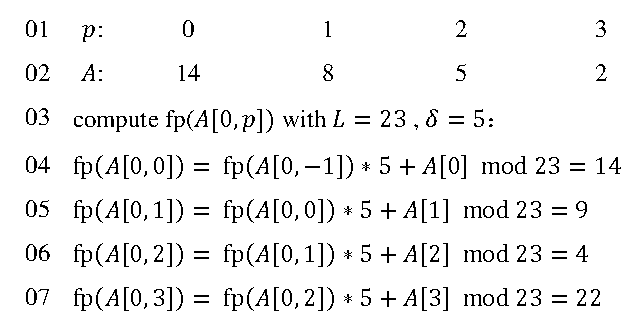
\includegraphics[width = 0.9\columnwidth]{example2.pdf}
	
	\caption{An example for calculating fingerprints by Karp-Rabin fingerprinting function.}
	
	\label{fig:example2}
	
\end{figure}

Methods A and B check equality of two integer arrays by computing and comparing their fingerprints. In our programs, we select the Karp-Rabin fingerprinting function to compute the fingerprints in need. As depicted in Fig.~\ref{fig:example2}, the fingerprint of $A$ is calculated according to Formulas~\ref{formula:1}-\ref{formula:2}, where $L$ is a prime and $\delta$ is an integer randomly chosen from $[1, L)$. It should be noticed that two equal arrays must have an identical fingerprint, but the inverse is not always true. Fortunately, the error probability can be reduced to a negligible level by setting $L$ to a large value.

\begin{formula} \label{formula:1}${\sf fp}(A[0, -1]) = 0$. 
\end{formula}

\begin{formula} \label{formula:2}${\sf fp}(A[0, i]) = {\sf fp}(A[0, i - 1]) \cdot {\delta} + A[i]\mod L$ for $i \ge 0$.
\end{formula}



\section{Experiments} \label{sec:experiments}

For implementation simplicity, we engineer DSA-IS and DSA-IS+ by the STXXL's containers~(vector, sorter, priority queue and stream). The experimental platform is a desktop computer equipped with an Intel Xeon E3-1220 V2 CPU, 4GiB RAM and 500GiB HD. All the programs are complied by gcc/g++ 4.8.4 with -O3 options under Ubuntu 14.04 64-bit operating system. In our experiments, three performance metrics are investigated for the programs running on the corpora listed in Table~\ref{tbl:corpora}, where each metric is measured as a mean of two runs.

\begin{itemize}
	\item construction time~(CT): the running time, in units of microseconds per character.
	\item peak disk use~(PDU): the maximum disk space requirement, in units of bytes per character.
	\item I/O volume~(IOV): as the term suggests, in units of bytes per character.
\end{itemize}

%Table
\renewcommand\arraystretch{1.3}
\begin{table}[!h]
	\caption{Corpus, $n$ in Gi, 1 byte per character} 
	\label{tbl:corpora}
	\centering
	\begin{tabular}{|l|c|c|p{5cm}|}
		\hline
		Corpora & \multicolumn{1}{c|}{$n$} & \multicolumn{1}{c|}{$\|\Sigma\|$} & Description \\\hline
		guten & 22.5 & 256 & Gutenberg, at \url{http://algo2.iti.kit.edu/bingmann/esais-corpus}.\\\hline 				
		enwiki & 74.7 & 256 & Enwiki, at \url{https://dumps.wikimedia.org/enwiki}, dated as 16/05/01. \\\hline	
		proteins & 1.1 & 27 & Swissprot database, at \url{http://pizzachili.dcc.uchile.cl/texts/protein}, dated as 06/12/15. \\\hline
		uniprot & 2.5 & 96 & UniProt Knowledgebase release 4.0, at \url{ftp://ftp.expasy.org/databases/.../complete}, dated as 16/05/11. \\\hline
	\end{tabular}
\end{table}

\subsection{Building Performance}

\begin{figure*}[t]
	\centering
	\subfigure[enwiki]{
		\begin{minipage}[b]{0.45\textwidth}
			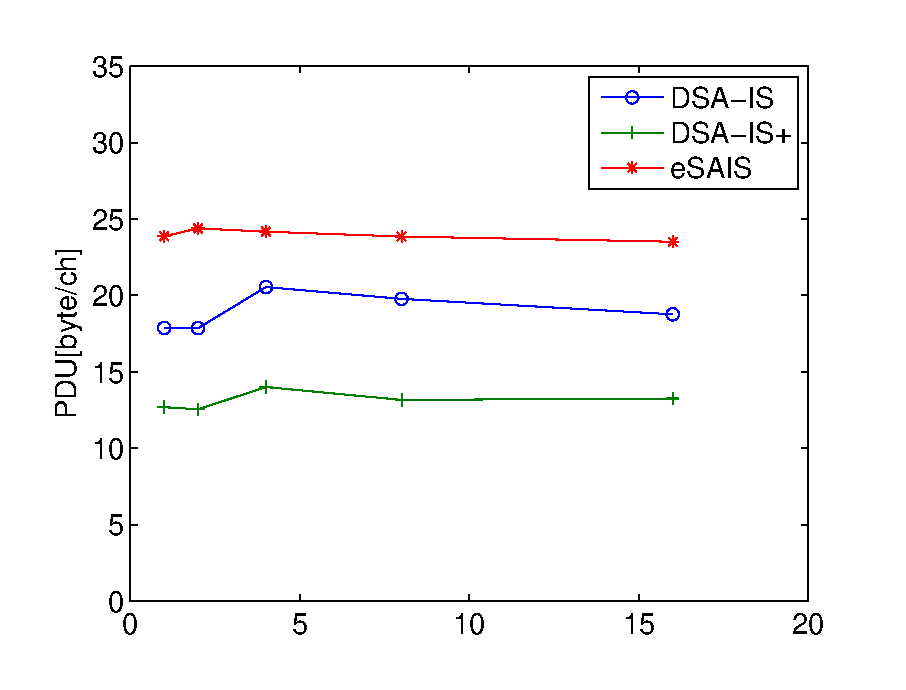
\includegraphics[width=1\textwidth]{construction_pdu_enwiki} \\
			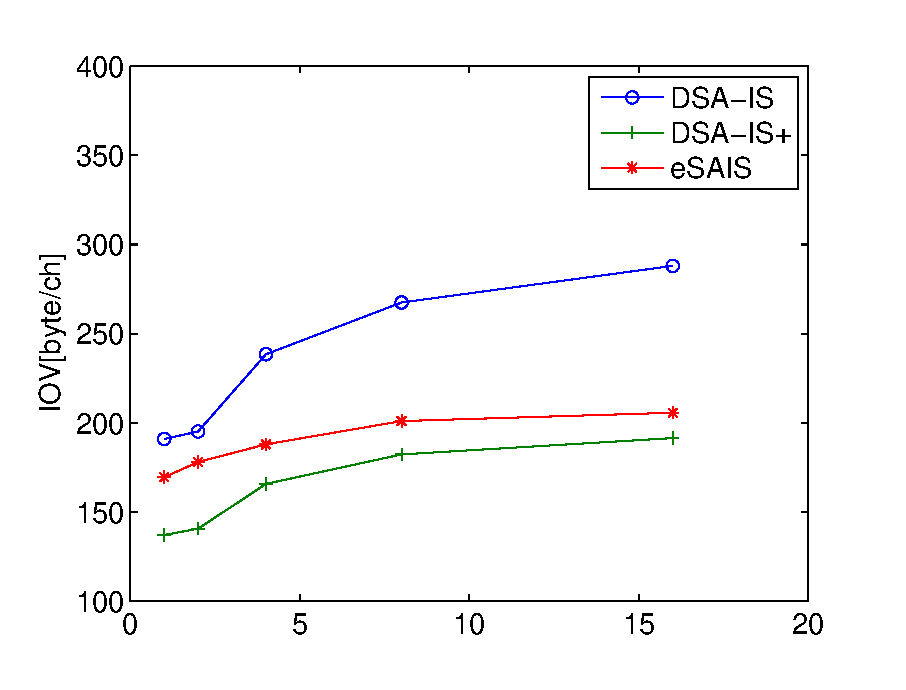
\includegraphics[width=1\textwidth]{construction_iov_enwiki} \\
			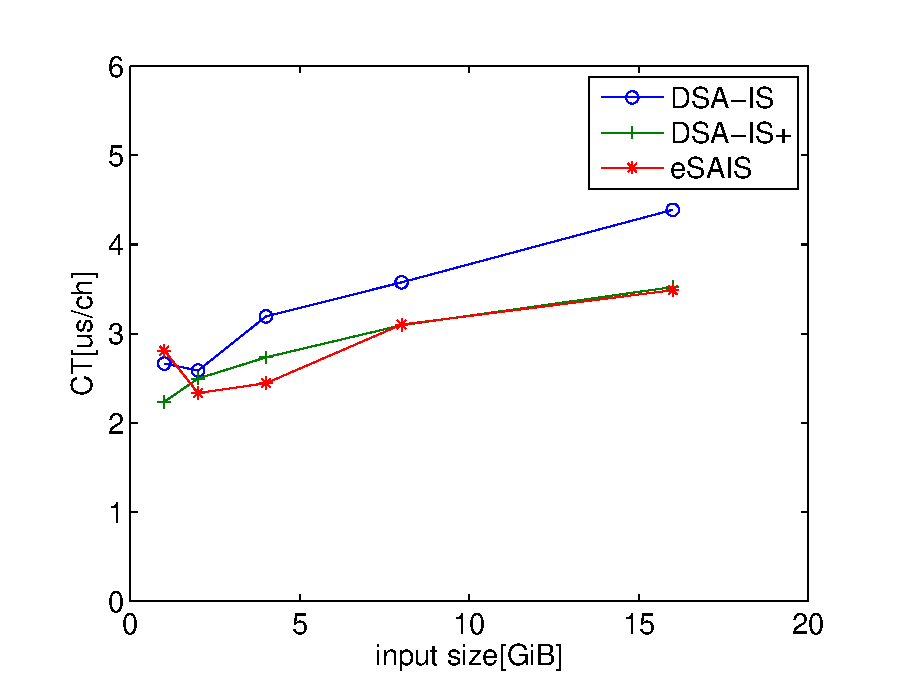
\includegraphics[width=1\textwidth]{construction_ct_enwiki}
		\end{minipage}
	}
	\subfigure[guten]{
		\begin{minipage}[b]{0.45\textwidth}
			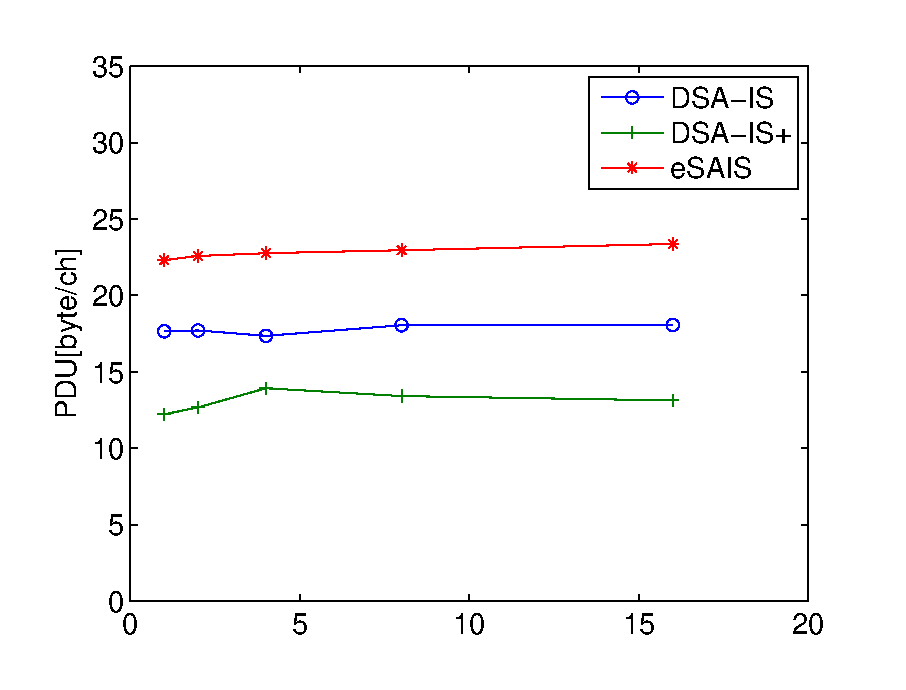
\includegraphics[width=1\textwidth]{construction_pdu_guten} \\
			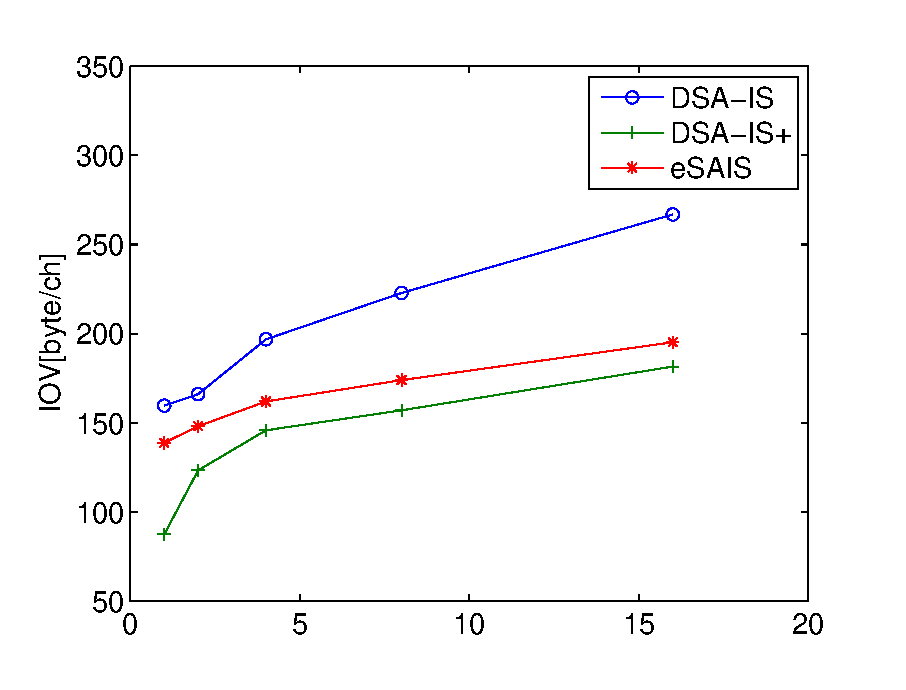
\includegraphics[width=1\textwidth]{construction_iov_guten} \\
			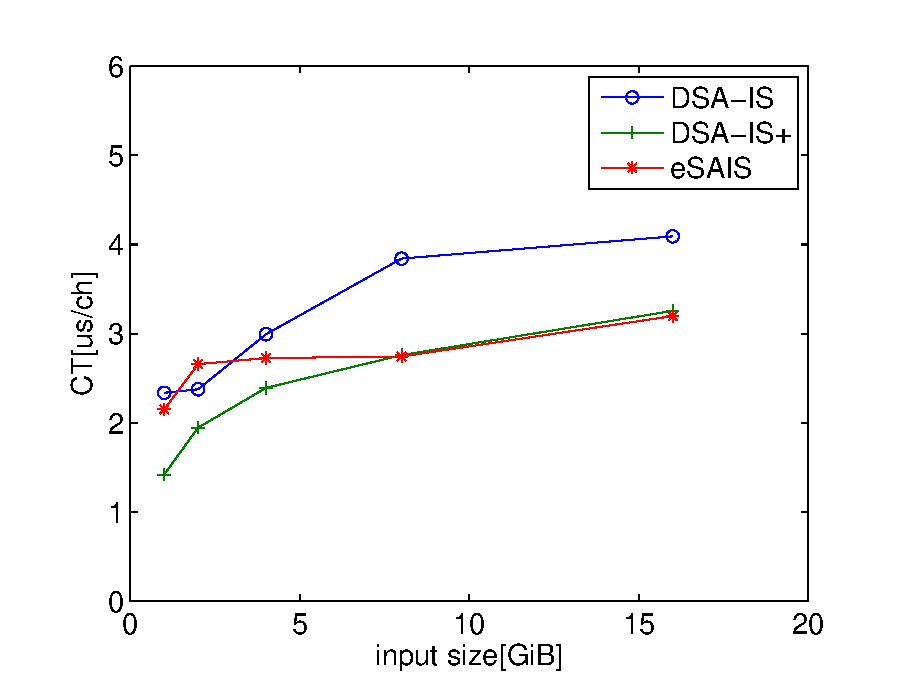
\includegraphics[width=1\textwidth]{construction_ct_guten}
		\end{minipage}
	}
	\caption{A comparison of DSA-IS, DSA-IS+ and eSAIS on guten and enwiki in terms of peak disk usage, I/O volume and construction time, where $D = 4$ and the input size varies in \{1, 2, 4, 8, 16\} GiB. }
	\label{fig:construction_performance1}
\end{figure*}

% Table
\begin{table*}%
	\caption{A Comparison of Reduction and Induction I/O Volumes Amongst DSA-IS, DSA-IS+ and eSAIS on enwiki}
	\label{tbl:volume_cmp}
	\centering
	\begin{tabular}{|c|c|c|c|c|c|c|c|c|c|c|c|c|}
		\hline
		\multicolumn{1}{|c}{} & \multicolumn{4}{|c|}{eSAIS} & \multicolumn{4}{c|}{DSA-IS} & \multicolumn{4}{c|}{DSA-IS+ ($D = 4$)}\\\hline
		\hline
		Size & Red. & Ind. & Total & Ratio & Red. & Ind. & Total & Ratio & Red. & Ind. & Total & Ratio\\\hline
		1G & 36.6 & 132.8 & 169.4 & 0.27 & 81.3 & 109.6 & 190.9 & 0.74 & 45.4 & 91.7 & 137.1 & 0.33\\\hline
		2G & 36.0 & 141.9 & 177.9 & 0.25 & 83.5 & 111.6 & 195.1 & 0.75 & 47.2 & 93.4 & 140.6 & 0.34\\\hline
		4G & 35.6 & 152.1 & 187.7 & 0.23 & 94.3 & 144.1 & 238.4 & 0.65 & 54.1 & 111.5  & 165.6 & 0.33\\\hline
		8G & 35.2 & 165.7 & 200.9 & 0.21 & 107.8 & 159.6 & 267.4 & 0.68 & 60.1 & 122.1 & 182.2 & 0.33\\\hline
		16G & 35.0 & 172.1 & 207.1 & 0.20 & 121.9 & 166.1 & 288.0 & 0.73 & 62.7 & 128.7 & 191.4 & 0.33\\\hline
	\end{tabular}
\end{table*}%

Because fSAIS is not available online, we use eSAIS as a baseline for analyzing the performance of DSA-IS and DSA-IS+. Fig.~\ref{fig:construction_performance1} shows a comparison between the programs for these three algorithms in terms of the investigated metrics. As depicted, the program for DSA-IS requires less disk space than that for eSAIS when running on "enwiki" and "guten". In details, the peak disk use of DSA-IS and eSAIS are around $18n$ and $24n$, respectively. However, eSAIS runs much faster than DSA-IS due to the different I/O volumes. In order for a deep insight, we collect in Table~\ref{tbl:volume_cmp} the statistics of their I/O volumes in the reduction and induction phases. As can be seen, although DSA-IS and eSAIS have similar performances when sorting suffixes in the induction phase, the latter consumes much less I/O volume than the former when sorting substrings in the reduction phase. More specifically, the mean ratio of induction I/O volume to reduction I/O volume are $0.23$ and $0.71$ for them, respectively. We can also see from the same figure that DSA-IS+ achieves a substantial improvement against DSA-IS, it runs as fast as eSAIS and takes half as much disk space as the latter. This is because the reduction I/O volume for DSA-IS+ is only half as much as that for DSA-IS (Table~\ref{tbl:volume_cmp}). Notice that the new substring sorting and naming methods adopted by DSA-IS+ take effect when most of the S*-type substrings are short. From our experiments, given $D = 8$, the ratio of long S*-type substrings in the investigated corpus nearly approaches one hundred percent, indicating that these methods are practical for real-world datasets.

\subsection{Checking Performance}

For evaluation, we integrate Method B into DSA-IS+ to constitute "Solution A" and compare it with "Solution B" composed of eSAIS and the existing checking method in~\cite{Dementiev2008a}. Fig.~\ref{fig:verification_performance} gives a glimpse of the performance of two solutions on various corpora. It can be observed that, the time, space and I/O volume for verification by Method B is negligible in comparison with that for construction by DSA-IS+, while the overhead for checking SA in Solution B is relatively large. Table~\ref{tbl:breakdown_solutionb} shows the performance breakdown of Solution B, where the checking time is one-fifth as the running time of the plain eSAIS and the peak disk use for verification is also a bit larger than that for construction. As a result, the combination of DSA-IS+ and Method B can build and check an SA in better total time and space.

\begin{figure}[t]
	\centering
	\subfigure{
		\label{subfig:verification_pdu}
		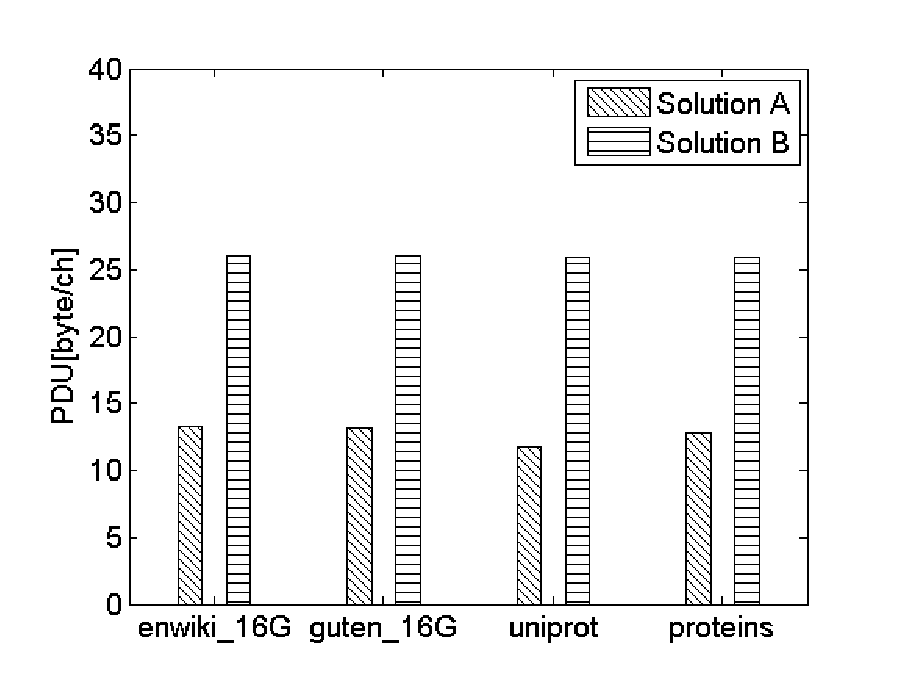
\includegraphics[width = 0.9\columnwidth]{verification_pdu}
	}
	\hfil
	\subfigure{
		\label{subfig:verification_iov}
		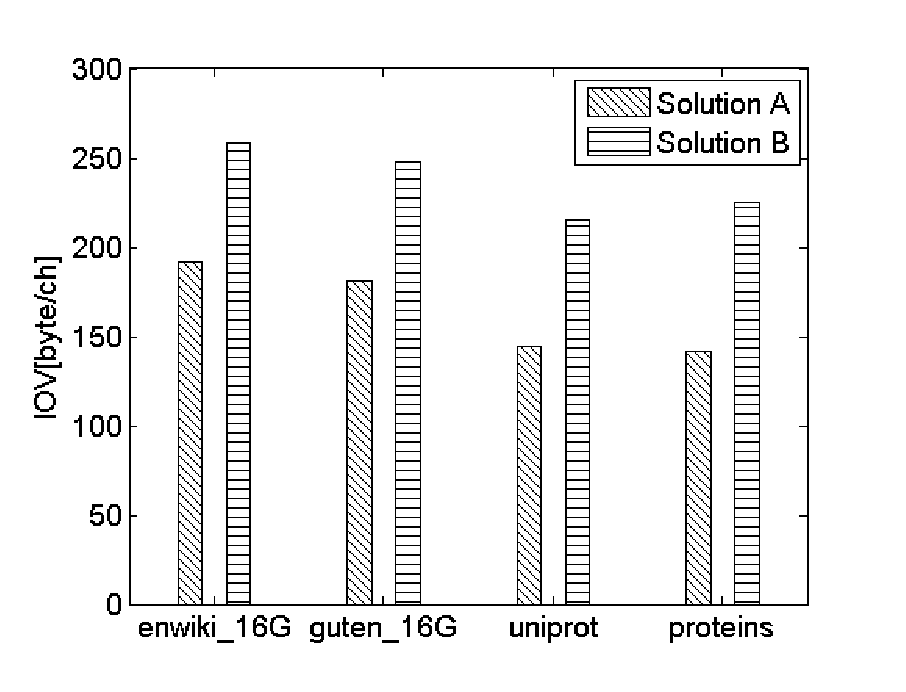
\includegraphics[width = 0.9\columnwidth]{verification_iov}
	}
	\hfil
	\subfigure{
		\label{subfig:verification_ct}
		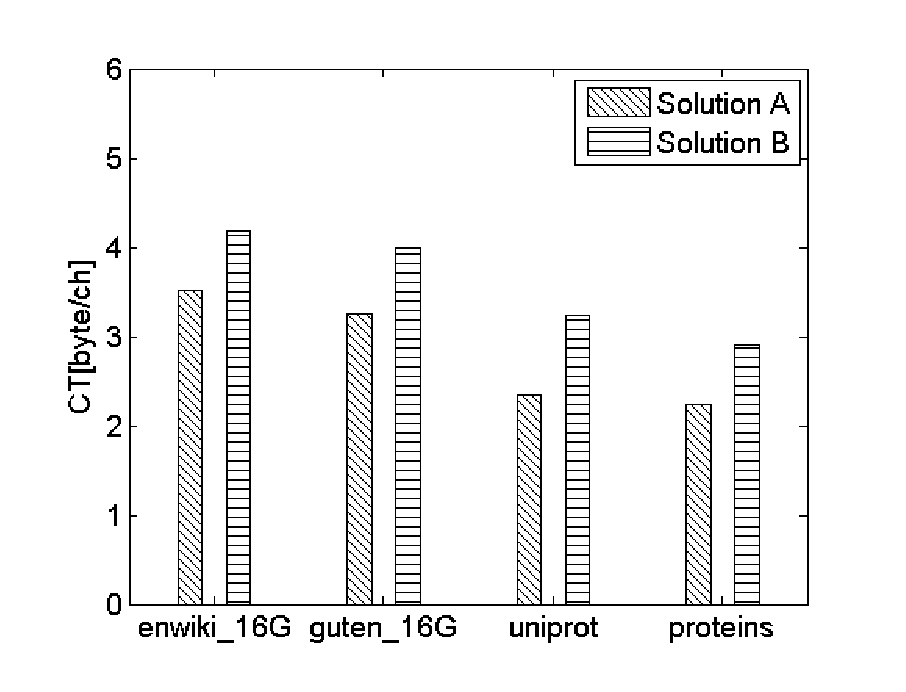
\includegraphics[width = 0.9\columnwidth]{verification_ct}
	}
	\caption{A comparison of Solutions A and B on various corpora in terms of peak disk usage, I/O volume and construction time, where $D = 4$.}
	\label{fig:verification_performance}
\end{figure}

% Table
\begin{table}%
	\caption{Performance Breakdown of Solution B on various Corpora}
	\label{tbl:breakdown_solutionb}
	\centering
	\begin{tabular}{|c|c|c|c|c|c|c|}
		\hline
		\multirow{2}{*}{Corpus} & \multicolumn{3}{|c}{checking} & \multicolumn{3}{|c|}{building} \\\cline{2-7}
		& PDU & IOV & CT & PDU & IOV & CT \\\hline
		enwiki\_16G & 26.0 & 53.0 & 0.71 & 23.5 & 205.6 & 3.49 \\\hline
		guten\_16G & 26.0 & 53.0 & 0.79 & 23.4 & 195.2 & 3.20 \\\hline
		uniprot & 25.9 & 53.0 & 0.74 & 22.7 & 162.0 & 2.50 \\\hline
		proteins & 25.9 & 53.0 & 0.58 & 24.1 & 172.3 & 2.33 \\\hline
	\end{tabular}
\end{table}%

According to Corollary~\ref{corollary:2}, Method A must check both $sa^*$ and $sa$ to accomplish verification. Similar to Method B, the overhead for checking $sa$ is mainly caused by fingerprint calculations and thus can be neglected. On the other hand, we can apply the method proposed in~\cite{wu2017} to ensure the correctness of $sa^*$ within sorting complexity, where the time and space in need is proportional to the number of S*-type characters in $x$. Because the ratio of S*-type characters to all in $x$ is commonly one-third in real-world datasets, the checking process for $sa^*$ will not become the bottleneck for Method A. To achieve a higher speed, we can also parallelize the checking processes for $sa$ and $sa^*$ using more computing resources.

\subsection{Discussion}

Rather than designing an I/O layer for efficient I/O operations, we currently use the containers provided by the STXXL library to perform reading, writing and sorting in external memory, these containers do not free the disk space for storing temporary data even if it is not needed any more, leading to a space consumption higher than our expectation. This is an implementation issue that can be solved by storing the data into multiple files and deleting each file when it is obsolete. In this way, our program can be further improved to achieve a space performance comparable to fSAIS. 

\section{Conclusion} \label{sec:conclusion}

In this paper, we proposed two methods that enable any IS suffix sorting algorithm to build and check SA simultaneously. In particular, the probabilistic algorithm designed by the second method is rather lightweight in terms of that it takes negligible time and space compared with the existing IS suffix sorting and checking algorithms. We also made an attempt to improve the space performance of DSA-IS using new substring sorting and naming methods. The experimental results shows that our program for the adapted algorithm DSA-IS+ runs as fast as that for eSAIS and requires only half as much disk space as the latter on various real-world datasets. We also showed that the space performance of this program can be further optimized using some optimization techniques. In our next paper, we will propose another disk-based suffix sorting algorithm that takes only $1n$ work space to run.



\bibliographystyle{IEEEtran}
\bibliography{IEEEabrv,bibfile}

\end{document}
